\documentclass[../main.tex]{subfiles} 

\begin{document}
\DndDropCapLine{T}{he Frontier.} A desert wasteland, hostile,
inhospitable, indomitable; a land shrouded in rumors --
strange creatures, otherworldly elementals,
warrior tribes...

The outside world knows practically nothing of this strange desert,
sleeping at the north-west edge of Vilterra. The Frontier rejected both the Elven
and Draconic lords in the ancient past or the nations and empires of the present
day, and remains shrouded in danger and intrigue.

\section{Geography}
Surrounded by mountains and hills, the Frontier is very much like a valley.
With not a single dorp of water, the inner regions are completely inhospitable.
By this, the Frontier is separated into the \emph{Outer} and \emph{Inner}
Frontier.

\subsection{Water}
For the most part, surface water is nonexistent in the Frontier. However,
that is not to say that there aren't \emph{any} water whatsoever.
Water from the Crown of the World gathered at the seasonal lake \emph{Kelibo},
and underground reservoirs are the most important water sources of desert
life.

However, the position and seasonal nature of
Kelibo makes it unsuitable for permanent residence, and the size of the
groundwater reservoir and the hostile surface made extracting water impractical.

%%%%%%%%%%%%%%%%%%%%%%%%%%%%%%%%%%%%%%%%%%%%%%%%%%%%%%%%%%%%%%%%%%%%%%%
%                               Ecology                               %
%%%%%%%%%%%%%%%%%%%%%%%%%%%%%%%%%%%%%%%%%%%%%%%%%%%%%%%%%%%%%%%%%%%%%%%
\section{Ecology}
Lacking the most important ingredient of life, the Frontier desert has
almost no life sparing a couple cacti and bushes on the edges. However,
there are some exceptions, especially on the Outer Frontier.

\subsection{Animals and Plants}
Heat-tolerant plants such as cacti and bushes exists in the more
hospitable Outer Frontier.

Camels also exists there, brought in by settlers. Most are domesticated,
though some do roam areas protected from monsters by people.

\subsection{Hostile Life}
Because intelligent life exert such little influence over the area, the
Frontier (especially the Inner Frontier) is filled with monsters.

The Frontier monsters are mostly reptilian and insectoid.
Most, such as basilisks, came down from the mountains. Nagas,
Ankhegs, and other beasts fight each other for sustenance.

\subsubsection{Elementals}
The most apt description of these mysterious, hostile creatures is
the manifestation of the forces of nature. Their origin are unknown,
their actions are inexplicable, all that's known about them is that
they have occupied this land since recorded history, and that
they will attack anything that they come across.

The elementals of the Frontier desert are mostly Fire, Air, and Earth.

\subsection{Sandworms}
Perhaps the most spectacular of the legends of the Frontier is the \emph{Sandworms},
and they certainly live up to it.

They are beings of massive proportions, some hundreds of feet long.
Much of their life is spent underground, where they supposedly
sustain themselves on underground water. The few times they surface
are primarilly for hunting, sunlight, and air.

Ironically, their times of hunting is also when they are most
vulnerable. Sandworms are prone to being prayed upon by other monsters.
The Shai-al run also use this opportunity to tame them.

Interestingly, Sandworms are attracted by music. The reason of which is
unknown. The Shai-al run takes advantage of this to call upon them.

\subsection{Migration of Kelibo}
At the north of the Frontier lies a seasonal lake Kelibo. In late winter,
early spring, the water from the northern mountains flows down into the
lake, attracting all kinds of life.

Basilisks from the mountains follows this stream down to the Frontier,
and some are left unable to leave.

Notably, the sandworms, despite having a consistent supply of underground
water, also gathers aroudn Kelibo primarily for hunting.

Because the allure of water is too great, bloody battles ensues everytime
water fills the lake. The violent nature of this seasonal event earned it
the name \emph{the Red Spring}.

Intelligent life such as the red dragonbornes also joins the fray for
sandworms; likewise, the Shai-al run are also present for water and
defense of the sandworms.

\section{History}
Not much ocurred in the Frontier worth noting; for the most part, it has
remained populated only by monsters and elementals. Almost all settling
attempts have ended in failure.

\subsection{Serovan Terraforming}
Much like what the high elves did to the Aurabe region in the far south,
they attempted to use magic to terraform the inhospitable Frontier.
However, their attempts are nowhere near as successful as in the South;
A mysterious force completely voided all of their arcane arts.

\subsection{Desolate Wasteland}
After failed Serovan terraforming, for the remainder of their rule
(and perhaps much longer after that) the Frontier remained a land
of no intelligent life or permanent settlements.

\subsection{The Shai-al run}
It was not until after the Great Dragon War before intelligent
life attempted to conquer the Frontier once again -- the Shai-al run.

This mysterious group of blue dragonbornes seemingly appeared
out of nowhere. They do not have a culture of recording history,
thereby we have no record of their origin. Due to the timing
of their approximate appearance coinciding with the Great Dragon
War, it is speculated that they are nobles of the fallen Meneketes
empire.

To this day, the Shai-al run remains the only semblance of
occupation in the Inner Frontier.

\subsection{Asakhani Advances}
The most recent attempts at settling the Frontier is made by
the Asakhan Empire. As a relatively newborn nation striving to
project power across Vilterra, they set their sights on the
inhospitable Frontier as a demonstration of force.

The Asakhanis relied on their experience in the Aurabe:
sponsoring the people of the southern desert to make for the north,
taking with them tools, livestocks, and experience suited to settling dry areas.
So far, their attempts haev been restricted to the Outer Frontier,
where permanent settlements are set up, relying on support from
the Empire to the south.

%%%%%%%%%%%%%%%%%%%%%%%%%%%%%%%%%%%%%%%%%%%%%%%%%%%%%%%%%%%%%%%%%%%%%%%
%                          Intelligent Life                           %
%%%%%%%%%%%%%%%%%%%%%%%%%%%%%%%%%%%%%%%%%%%%%%%%%%%%%%%%%%%%%%%%%%%%%%%
\section{Intelligent Life}
Due to the harsh conditions of the Frontier, intelligent life is few and
far between. However, several exceptions stands out, braving the
harsh desert.

%%%%%%%%%%%%%%%%%
%  Shai-al run  %
%%%%%%%%%%%%%%%%%
\subsection{The Shai-al run}
\subsubsection{Overview}
By far the most notable of the intelligent races that inhabits the
Frontier is the assortment of blue-dragonborne tribes that collectively
call themselves the \emph{Shai-al run}. They are the only race that can
truly call this land home.

\subsubsection{Organization}
Rather than a single nation-state, the Shai-al run is more like a
collection of cooperative tribes, operating almost completely
independently.
\paragraph{Kelibo}
As with most creatures of the desert, the Shai-al run tribes makes a
annual migration to the lake of Kelibo, primarily to follow and protect the
sandworms. It is one of the only instances where all of the Shai-al run
work together.

\subsubsection{Way of Life}
\paragraph{Martial Culture}
To survive in the unforgiving Frontier, the people of Shai-al run
became adept at combat by necessity; both for fending of threats and
for monster-hunting.

Due to constantly hunting for monsters and fending off the wyvern-riding red
dragonbornes, Shai-al run warriors primarily use heavy or ranged weaponry,
some of which forged in Kelibo, most of which procured from monster remains.
\paragraph{Sandworms}
The most distinguishing trait of the Shai-al run is their taming
of the sandworms. The exact methods of taming a sandworm is known to very few;
it seems to have something to do with the Nu-cha flute -- another
symbol of Shai-al run culture
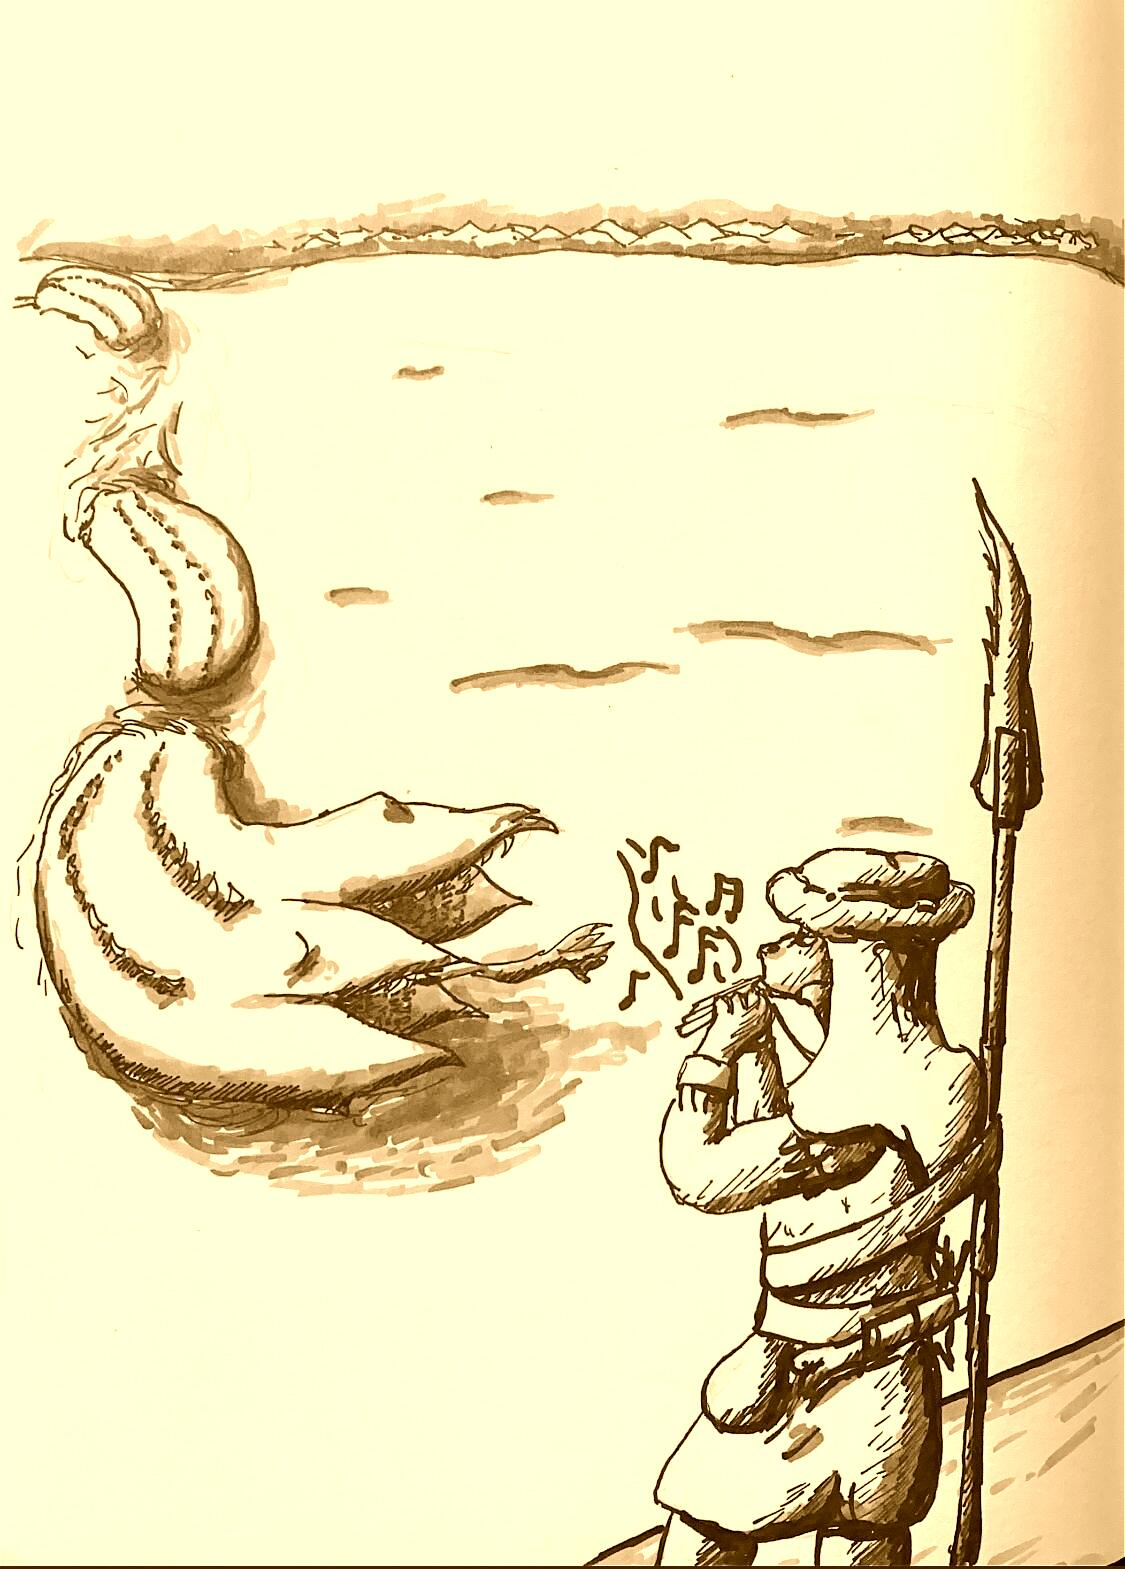
\includegraphics[width=\columnwidth]{charm_sandworm.jpeg}

\subsubsection{Conflict}
The Shai-al run tribes are known to be territorial. They are known to attack
Asakhani settlers that came too close to the Inner Frontier.

%%%%%%%%%%%%%%%
%  Outsiders  %
%%%%%%%%%%%%%%%
\subsection{Outsiders}
While the Shai-al run is the only permanent resident of the Frontier,
there are numerous peoples that, despite living elsewhere, frequent the area.

\subsubsection{Ironok}
While primarily residing in the mountain ranges to the west of the Frontier,
the Ironok goblins have a great prescence on the Frontier.

Similar to the Shai-al run,
the Ironok is a collection of cooperative Goblin tribes.

\subsubsection{Io-to}
The Shai-al run are not the only dragonborne seen on the Frontier.
Residing in the Northern mountains are the red dragonborne of \emph{Io-to}.
They are most famous for their mount -- wyverns.

\subsubsection{For the Sandworms}
Despite the Frontier being a hostile place with little to no natural resources,
these Outsiders risk their lives and the wrath of the Shai-al run for one thing
-- Sandworms.

The Ironok and Io-to hunts sandworms for medicine. This, of course, incurs
the wrath of the Shai-al run that rely on those sandworms to stay alive
in the arid and dangerous desert. As a result, bloody conflicts are very
frequent.

\subsubsection{Asakhani Settlements}
As a testament to the imperious reach of the Askhan Empire, settlers
dotted the edges of the Outer Frontier; Most of them are brought over
from the Aurabe desert, with one singular goal -- conquer the harsh
environments of the Frontier.

\end{document}
